\section{数値実験}\label{sec:results}
$\delta=0.05$、$\kappa=0.95$、有限配分$b/E\in\{0.4,0.6,0.8\}$を用いる。
8条件は$a\in\{0.3,0.6\}$、$u\in\{0.125,0.2\}$、$E=0.025$、
$c_\psi\in\{1,32\}$、$N=20$の組合せである。
追加2条件は$a=0.6$、$u\in\{0.25,0.4\}$、$E=0.05$、$c_\psi=1$、$N=12$とする。
各問題の全直列query上限は$c_\psi+4N+1$であり、全条件で$u>4E$を満たす。
$c_\psi$は費用モデルの感度パラメータであり、行列監査の単純な入力準備が
実機で32queryを必要とするという主張ではない。

\paragraph{候補と証明}
比較するのは$(1-x)^n$、$(1-x^2)^t$、上端零化したcosine-Taylor積
$(1-x)(1-0.72x^2)^t$、および古典low-pass Chebyshevに$1-x$を掛けた
\[
 (1-x)\frac{T_{n-1}((2x-1-v)/(1-v))}
                  {T_{n-1}(-(1+v)/(1-v))},\qquad
 v\in\{.04,.08,.16,.28,.42,.60,.78\}
\]
である。次数は常にGram変数$x$で数え、同じ規約でsignal queryへ換算する。
報告する各候補について正規化、目標正値性、バイアスを連続証明する。
最適化候補の初期格子は目標17点、tail 65点、support 129点で、より密な格子に対して
最大3回exchangeする。設計バイアスは$0.98b$、連続証明は$0.99b$とし、$0.01b$を
実現誤差用に残す。有限格子の最適解でも証明に失敗すれば選ばない。
したがって選択上界は試した証明済み候補の最良値であり、独立dual下界が最適性の差を
保証する。

\begin{table}[tb]
\centering\small
\begin{tabular}{rrrrrlrrr}
\toprule
$a$ & $u$ & $E$ & $c_\psi$ & $n$ & Response & $b$ & $J^{\rm up}$ & Gap \\
\midrule
0.30 & 0.125 & 0.025 & 1 & 8 & LP & 0.015 & 1.79e+08 & 9.5\% \\
0.30 & 0.125 & 0.025 & 32 & 8 & LP & 0.015 & 3.47e+08 & 9.5\% \\
0.30 & 0.200 & 0.025 & 1 & 8 & LP & 0.020 & 1.71e+09 & 23.9\% \\
0.30 & 0.200 & 0.025 & 32 & 8 & LP & 0.020 & 3.31e+09 & 16.2\% \\
0.60 & 0.125 & 0.025 & 1 & 4 & LP & 0.015 & 3.27e+06 & 21.4\% \\
0.60 & 0.125 & 0.025 & 32 & 4 & LP & 0.015 & 9.19e+06 & 3.7\% \\
0.60 & 0.200 & 0.025 & 1 & 4 & LP & 0.015 & 1.02e+07 & 7.5\% \\
0.60 & 0.200 & 0.025 & 32 & 5 & LP & 0.015 & 2.72e+07 & 5.6\% \\
0.60 & 0.250 & 0.050 & 1 & 2 & Cheb. & 0.030 & 5.1e+05 & 4.9\% \\
0.60 & 0.400 & 0.050 & 1 & 3 & LP & 0.030 & 1.98e+06 & 7.4\% \\
\bottomrule
\end{tabular}

\caption{事前情報だけからの選択。$n$はGram次数、LPは証明済み最適化多項式、Cheb.は
試した格子内のChebyshev応答。Gapは$100(J^{\rm up}/\min J^{\rm lo}-1)$であり、
上端零化クラス・次数上限・有限配分格子に対する値で、全量子推定器に対する値ではない。}
\label{tab:selection}
\end{table}
選択費用の、制限した最適費用下界に対する比は$1.0372$から$1.2394$である。
大半は結合LPの応答だが、$a=0.6,u=0.25,E=0.05$ではChebyshev候補を選ぶ。
新しく最適化した族を常に優先する実装にはしていない。
べき乗とChebyshev候補は全10条件で証明できた。
quartic-powerとcosine-Taylorは、今回の難しい条件群で、探索した次数・パラメータ範囲
に証明済み可行候補を返さなかった。これは全調整に対する不可能性証明ではない。
試したべき乗候補の費用上界は、選択上界の約$1.44$から$4.36$倍だった。
共通モデルの保証費用の比較であり、実測実行時間の高速化ではない。

\begin{figure}[tb]
\centering
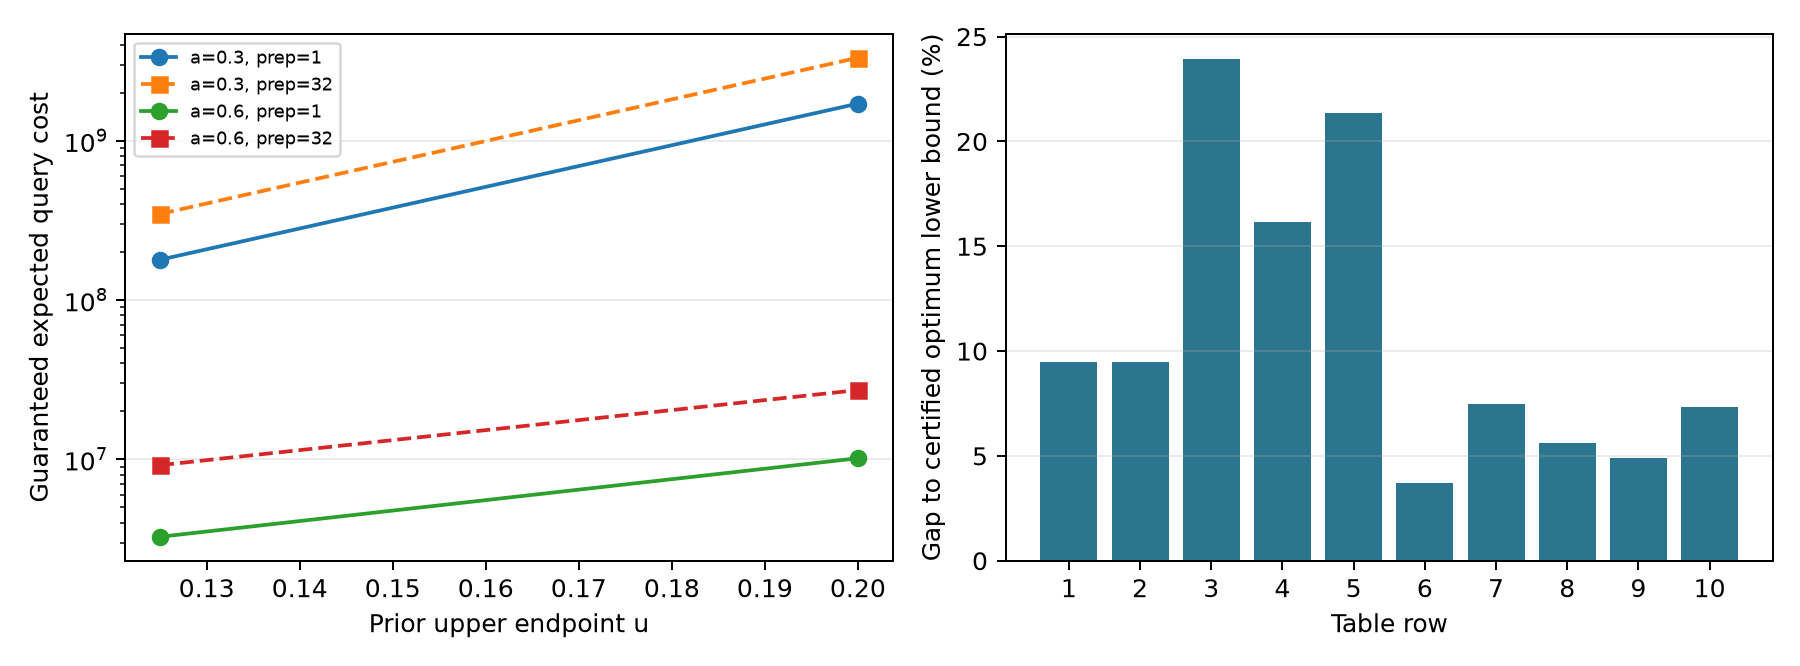
\includegraphics[width=\linewidth]{../../figures/selection_costs.png}
\caption{保証された期待query費用と事後的最適性Gap。
準備費用が違う条件は別の指定問題であり、各問題内では全候補の上限とoracle規約を揃える。}
\end{figure}

\paragraph{準備費用による切替}
$a=0.6,u=0.2,E=0.025,b=0.015$では、準備費用1で次数4、準備費用32で次数5を選ぶ。
受理コピー数は同一であり、後者の高い保証受理確率が、高価な準備の際に追加queryを
相殺する。理想多項式応答の厳密透過率区間から切替点を包囲でき、表示保証費用の交点は準備query単位で
約$12.34$となる。これは二つの固定多項式の比較であり、中間の全準備費用でこの二つだけが
最適候補になるとの主張ではない。

\begin{figure}[tb]
\centering
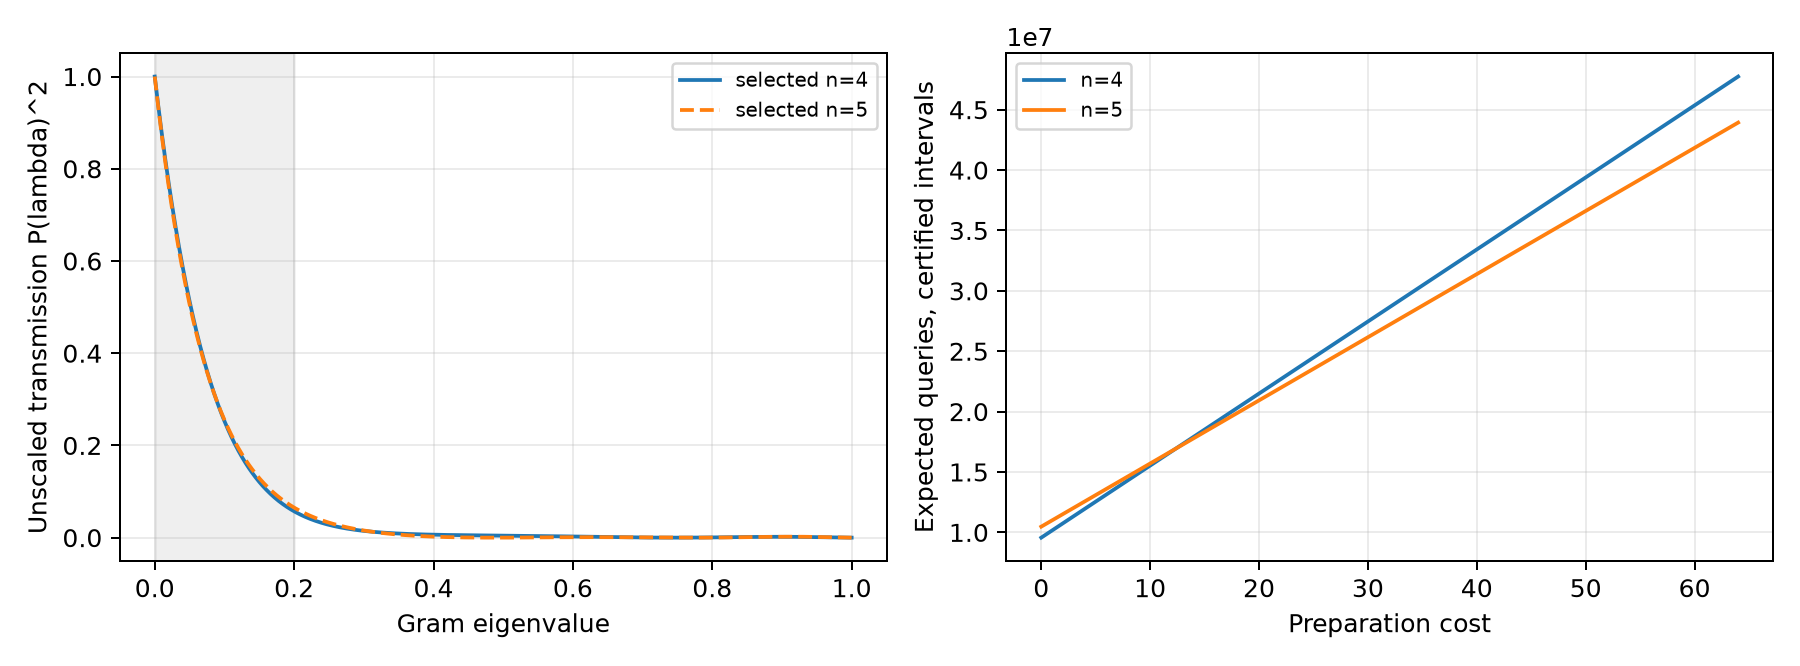
\includegraphics[width=\linewidth]{../../figures/selection_crossover.png}
\caption{同じ事前情報・バイアス配分に対する二応答。灰色は事前区間。
透過率包囲が費用の細い帯を与え、準備費用の増加で順序が変わる。}
\end{figure}

\paragraph{事前区間幅の費用}
命題\ref{prop:prior}の無制約上界を、証明済み多項式透過率が超えないことを確認した。
$a=0.3,E=0.025,c_\psi=1$では、$u=0.125$から$0.2$への拡大で、選択保証費用は
約$1.79\times10^8$から$1.71\times10^9$ queryへ増える。
大きい絶対費用は実用性の証拠ではなく、この頑健平均推定規約の限界を示す。

\begin{figure}[tb]
\centering
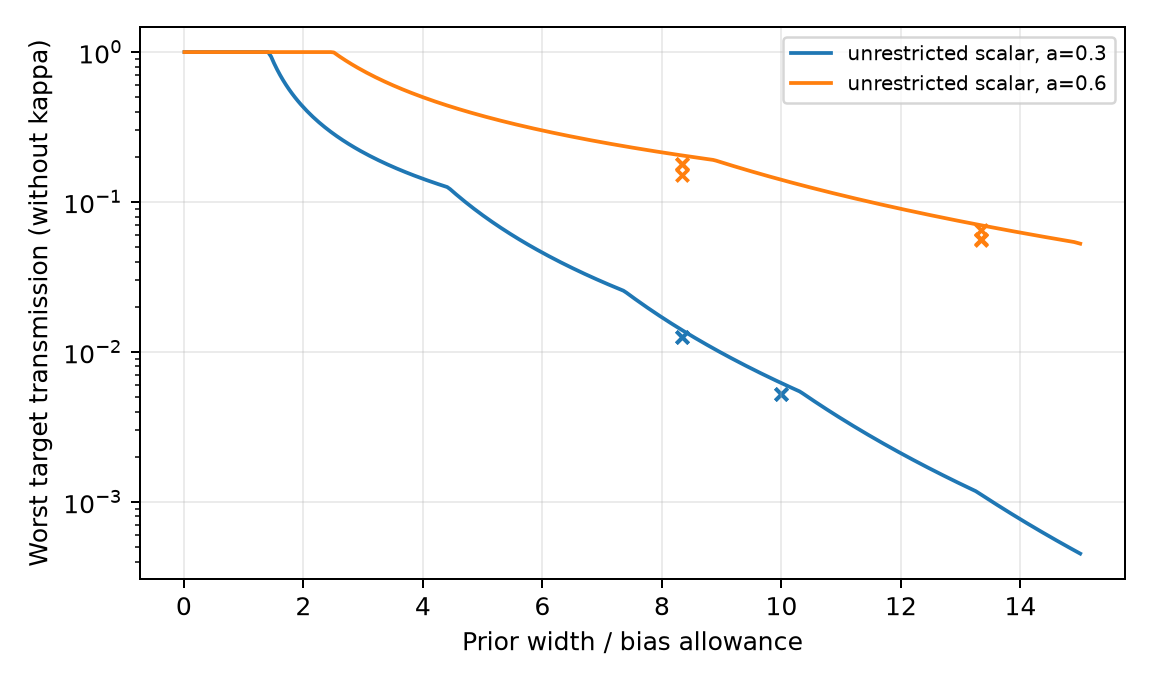
\includegraphics[width=.72\linewidth]{../../figures/selection_prior_limit.png}
\caption{事前区間幅／許容バイアスに対する無制約透過率上界と、証明済み多項式の値（×）。
両者から共通余裕$\kappa$を除いている。}
\end{figure}

\paragraph{位相・行列監査}
選択した全10多項式で位相合成に成功した。
保存位相から連続証明した最大振幅誤差は$3.63\times10^{-16}$で、全候補が予約バイアスを
満たす。実装成功下界への補正による費用増加率は$1+1.4\times10^{-14}$未満である。
これらは理想signal規約の結果であり、実機回転合成や雑音encodingへの保証ではない。

各選択に対し8次元正行列$B$を生成し、入力を固定計算基底$\ket0$とする。
生成側のHouseholder回転で重なりpromiseを制御するが、設計側には真の固有値も
その回転も与えない。各組の一例は最小値の$10^{-7}$上に励起値を置く。
16×16 signal行列へ全位相を適用し、32×32抽出ユニタリも明示的に構成した。
多項式目標との最大行列応答誤差は$5.55\times10^{-16}$、最大ユニタリ残差は
$6.33\times10^{-15}$であった。これはoracleの行列シミュレーションであり、物理ゲート合成ではない。

seed 20261027の独立なスカラー入力1,000例で、バイアスと受理確率の境界を確認した。
行列例ではseed 20261028のBernoulli・負の二項分布による集約標本計2,000反復を行い、
要求誤差に対するconfidence failureは零だった。
確率保証は定理から得るもので、有限観測で零だったことは整合確認にすぎない。
全係数・位相・入力行列・標本設定・厳密証明データを同梱する。
